\documentclass[12pt,a4paper, twoside]{article}
\usepackage[T1]{fontenc}
\usepackage{fancyhdr}
\usepackage[utf8]{inputenc}
\usepackage[french]{babel}
\usepackage{color}
\usepackage{graphicx}
\usepackage{hyperref}
\usepackage[left=3cm,right=3cm,top=2cm,bottom=2cm]{geometry}
\usepackage{array}
\pagestyle{fancy}
\setlength{\headheight}{12pt}
\usepackage[acronym]{glossaries}
\makeglossaries
\begin{document}

\begin{titlepage}
    \begin{minipage}[t]{0.48\textwidth}
        
\includegraphics[height=1.01cm]{logolemansU.png}
    \end{minipage}
    \hfill
    \begin{minipage}[t]{0.25\textwidth}
        
\includegraphics[height=1.6cm]{logo_IC2.png}
    \end{minipage}
    
    \vspace{2cm}
    \begin{center}
        \Large\textbf{Le Mans Université}\\
        \vspace{0.5cm}
        Licence Informatique 2ème année\\
        Module 17UF02 Rapport de Projet\\
        \vspace{0.5cm}
        \Large\textbf{Titre du projet}\\
        \vspace{1cm}
        {\large Noms des auteurs}\\
        \vspace{0.5cm}
        {\normalsize \today} 
    \end{center}
\end{titlepage}

\newpage
\tableofcontents
\newpage
\abstract{
    Ceci est le texte de mon résumé...
}
\section{Introduction}

\emph{Cette introduction présentera le sujet qui sera traité et le travail avec une présentation du plan adopté}\\
Dans le cadre d'un projet de notre fin d'année de L2 informatique, le type de jeu vidéo créer est un jeu de rôle qui se joue en tour par tour en faisant affronter des créatures fantastiques a l’instar du jeu phare de Nintendo nommé « Pokemon ».\\
Ce projet a été réaliser en langage C avec la librairie SDL et contrairement a son inspiration , le jeu ne se passe pas dans un pays tous droit sorti de l’imaginaire d’une personne mais bel et bien au sein du bâtiment de l’Institut Claude Chappe, Vous incarnerez un nouvel étudiant rentrant en première année et affronterez d'autres étudiants et enseignants chercheurs déjà installés dans le bâtiment a travers des duels de ICmon.\\ 

En première partie, nous allons expliquer comment nous avons conçu le jeu, une présentation général et détaillé de l’univers dans lequel il se situe, son histoire ainsi que celui du joueur communément appeler son « lore » .
Ensuite sa direction artistique c’est a dire tous l’aspect graphique seront expliciter , avec quels logiciels les sprites des Icmons, du joueur et des niveaux ont été esquisser et enfin toutes les possibilités offertes au joueur pendant son aventure.\\

Puis nous parlerons de l’organisation, quelles missions a été confié pour chaque personne du groupe et sous quels deadline devaient-elles être rendu ,tous ceci a été planifié grâce a un diagramme de Gantt que nous avons réalisé.\\

En troisième partie nous expliquerons la gestion des Icmons , comment ils ont été générés et comment la gestion des duels a été réalisé, puis nous parlerons de la gestion des bases de données, comment les données des Icmons et le jeu ont été sauvegardé puis chargé et ensuite réutiliser de nouveau.\\

Puis nous aborderons la gestion de la carte, comment le joueur se déplace dans l'espace et comment la caméra le suit. et lorsqu'il rencontre un obstacle, une collision doit se produire.\\

Et enfin nous mettre en évidence la rendu du jeu , les sprites que nous avons créer doivent être implémenté directement dans le code, le système de combat c’est a dire les points de vie décrémenter lorsqu’une attaque est subie ,devrait être cohérent avec ce que le joueur voit sur l’écran et pour finir l’interface par quel moyen l’interface du jeu a été conçu, de quelle façon le joueur change de fenêtre lorsque tel bouton est appuyé\\\\
\lfoot\fancyfoot{\footnotesize *Pokemon:le jeu sera présenter dans la suite du rapport\\*Sprite: image 2D utilisé dans les jeux vidéos\\*ICmon: contraction de l'expression « Institut Claude chappe » et « Monstre »\\*Lore: histoire d'un jeu vidéo\\*deadline: date limite\\}
\newpage
\section{Conception}
    \subsection{Présentation du jeu}
        ICPocket est un jeu de rôle basé sur l'univers des jeux vidéos « Pokémon » développés par GAME FREAK et publiés par Nintendo.
        Le jeu met le joueur dans la peau d'un étudiant de la faculté d'informatique du Mans et d'un dresseur de petites créatures nommées les \emph{ICMons}.
        Cet étudiant, qui vient tout juste d'arriver au sein de l'institut Claude Chappe pour sa première année de license, choisit son premier partenaire parmi quatre ICmons offerts par Louis, Nathan, Alban et William.
        \paragraph{}L'objectif du joueur est de devenir le maître de l'IC2 en remportant le tournoi annuel de la faculté : « le tournoi de l'IC2 », puis en faisant tombé son conseil des quatres et son champion. Pour cela, il devra se confronter à ses camarades et ses professeurs dans des duels d'ICMons : 
        des combats de type joueur contre ordinateur en tour par tour dans lequelles chaque partie envoit un ICMons parmi un maximum de six se battre contre l'autre, jusqu'à ce que l'un des combattants n'est plus aucun ICMons apte à se battre.
        Ces affrontements tactiques et imprévisibles pousseront le joueur à découvrir les forces et faiblesses de son équipe et à mettre en place la meilleure stratégie pour parvenir à la victoire.
        Toutefois, cela ne sera pas une tâche aisée, puisque la moindre défaite signifie que le joueur sera éliminé du tournoi et devra donc recommencer du début.

    \subsection{Direction artistique}
        En hommage aux jeux vidéos originaux de la série « Pokémon », nous avons fait le choix de nous inspirer de la direction artistique de la troisième génération de ces jeux : « Pokémon Rubis et Saphir ».
        Cette direction artistique est basée sur la 2D, avec des sprites pixelisées. \paragraph{} Pour la réalisation de la carte, nous avons utilisé les assets libre de droit disponible sur le site \href{https://kenney.nl/assets}{kenney.nl}. La carte a ensuite été assemblé par Alban et Louis. La plupart des sprites des ICMons ont été dessiné par William, Loup Picault (le goat), et Nathan. Les sprites restants ont été dessiné par intelligence artificielle.
        \paragraph{} Afin de limiter le nombre de sprites que nous avions à réaliser pour ce projet, nous nous sommes inspirés de la méthode d'affichage des sprites du fangame \href{https://infinitefusion.fandom.com/wiki/Pok%C3%A9mon_Infinite_Fusion_Wiki}{« Pokemon Infinite Fusion »}, dans lequelle durant un combat, les sprites de l'équipe du joueur sont retournés par symétrie axiale verticale, ce qui donne l'illusion d'un sprite \emph{de dos} tout en ayant qu'un seul sprite à utiliser.
        \begin{figure}[h!]
            \centering
            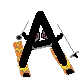
\includegraphics[width=0.22\textwidth]{../assets/Monsters/New Versions/A-ski.png}
            \label{fig:ICMon}
            \caption{Exemple de sprite pour un ICMon}
        \end{figure} 

    \subsection{Fonctionnalités}
        \emph{Dans cette partie, nous présenterons toutes les fonctionnalités disponibles dans le jeu} \\
        \paragraph{} Au lancement du jeu, le joueur peut personnaliser ses paramètres selon ses souhaits : les dimensions de la fenêtre d'écran, la vitesse du texte en jeu et le volume sonore. Après cela, il peut charger une partie déjà entamée, à condition qu'une telle partie existe dans les fichiers du jeu, ou bien débuter une nouvelle aventure. \paragraph{}
        Dans le cas d'une nouvelle partie, le joueur se vera alors proposé quatre ICMons et choisira celui qu'il préfère, puis arrivera sur la carte, à l'entrée du bâtiment IC2. Le joueur peut alors explorer la carte comme il le souhaite : hall d'accueil, salle de TD et amphitéâtre. Le joueur trouvera également en bas de l'escalier principal un drôle de personnage nommé <Insérer nom ici>.
        Le joueur peut discuter avec lui : <Insérer nom ici> proposera notamment au joueur de changer d'endroit pour commencer son prochain match du tournoi de l'IC2.
        \paragraph{} Puis l'affrontement commence. Le joueur et son opposant, controlé par l'ordinateur, envoient au combat l'ICMons se trouvant en tête de leurs équipes respectives. Chaque tour, les deux protagonistes choisissent une action parmi les deux suivantes : utiliser l'une des quatres attaques connues de leur ICMon, ou bien remplacer le combattant actuel par un autre encore apte dans leur équipe.
        Durant ce duel, différentes afflictions peuvent modifiées le cours de la partie. En effet, certaines attaques possèdent une chance plus ou moins grande d'empoisonner, de brûler, de rendre confus, d'apeurer ou d'altérer les forces du lanceur de la capacité et de l'adversaire. \paragraph{}
        Le combat continue jusqu'à ce que les ICMons d'un des dresseurs soient tous hors d'état de se battre. Si le joueur perd son duel, sa sauvegarde est supprimée et il doit recommencer une nouvelle partie pour tenter de battre son meilleur score, c'est-à-dire son nombre de victoire.
        Dans le cas contraire, le joueur peut, si il le souhaite, récupérer l'un des ICMons que son adversaire avait dans son équipe et l'ajouter à la sienne. Enfin, le joueur retourne dans le hall du bâtiment IC2 pour se préparer au prochain affrontement.
        La partie en cours est sauvegardée à la fin de chaque duel, en cas de victoire du joueur, afin qu'il puisse mettre en pause son aventure et la reprendre plus tard. \paragraph{}
        Au bout de quinze victoires consécutives, les cinqs derniers combats proposés au joueur seront contre le conseil des quatres, composé des quatres créateurs du jeu : Louis, Nathan, Alban et William, et l'affrontement ultime contre Mme Py, professeur à l'université du Mans en informatique et dans le cadre du jeu mâitresse de l'IC2.
        Si le joueur parvient à faire chûter Mme Py de son trône, il remporte la partie. 


\newpage
\section{Organisation}
Notre projet de jeu 2D a été développé selon une architecture modulaire rigoureuse, permettant une séparation claire des responsabilités entre les différents composants. Nous avons adopté un modèle de développement itératif, en commençant par implémenter les fonctionnalités essentielles du moteur de jeu avant d'ajouter progressivement des mécanismes plus complexes. L'organisation s'est articulée autour de trois axes principaux : la gestion du rendu graphique avec SDL, la logique de jeu et les structures de données, et enfin la synchronisation entre ces éléments via un gestionnaire de threads. Cette approche nous a permis de maintenir un code propre et maintenable, tout en facilitant le débogage et l'extension des fonctionnalités au cours du développement. Notre système de maps interconnectées avec mémorisation des positions du joueur illustre parfaitement cette approche modulaire, où chaque composant (Map, Player, Camera) remplit un rôle spécifique mais communique efficacement avec les autres.

\subsection{Planning Prévisionnel}
\begin{figure}[h]
    \centering
    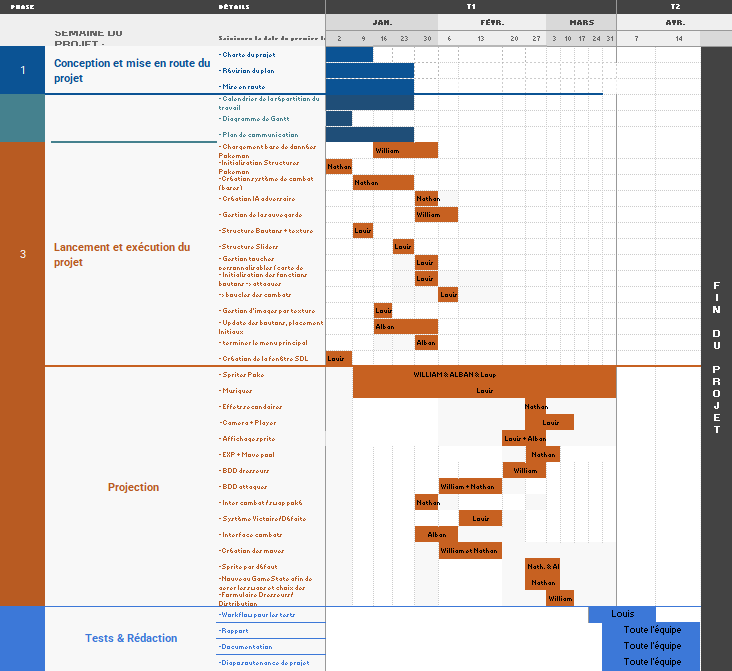
\includegraphics[width=0.75\textwidth]{GANTT.png}
    \label{fig:GANTT}
    \caption{Diagramme de Gantt}
\end{figure}

Notre planning prévisionnel a été établi dès le début du projet pour garantir une progression cohérente et le respect des délais. Nous avons divisé le développement en plusieurs phases distinctes, chacune avec des objectifs spécifiques et des livrables clairement définis. Cette approche structurée nous a permis d'identifier rapidement les tâches critiques et d'allouer les ressources nécessaires en conséquence. Grâce à des points de contrôle réguliers, nous avons pu ajuster notre planification en fonction des difficultés rencontrées et des avancées réalisées, assurant ainsi une gestion efficace du temps disponible jusqu'à l'échéance finale.

L'élaboration de notre planning prévisionnel s'est appuyée sur une méthode d'estimation collaborative où chaque membre de l'équipe a évalué le temps nécessaire pour les tâches relevant de son domaine d'expertise. Pour les composants interdépendants comme le système de transition entre maps et la gestion des déplacements du joueur, nous avons organisé des sessions de planification poker où les estimations individuelles étaient discutées pour atteindre un consensus. Cette méthode nous a permis d'identifier dès le départ les zones de risque potentiel, comme la synchronisation des threads ou la gestion des collisions, qui ont bénéficié d'une marge temporelle supplémentaire dans notre planning.

Notre diagramme de Gantt identifie clairement quatre jalons principaux : la finalisation de l'architecture de base (semaine 4), l'implémentation du système de combat (semaine 8), l'intégration complète des maps et des transitions (semaine 12), et les tests d'intégration finaux (semaine 15). Ces jalons ont servi de points d'ancrage pour nos réunions d'avancement et nous ont permis de mesurer objectivement notre progression par rapport aux objectifs initiaux. Une caractéristique importante de notre approche a été l'inclusion délibérée de périodes tampons après chaque jalon majeur, offrant la flexibilité nécessaire pour gérer les imprévus techniques inévitables dans le développement d'un jeu.

\subsection{Répartition des tâches}
La répartition des tâches s'est effectuée en fonction des compétences et des intérêts de chaque membre de l'équipe. Pour structurer notre travail et définir clairement les responsabilités, nous avons mis en place une matrice RACI complète. Cette matrice a permis d'identifier pour chaque tâche du projet qui était Responsable de son exécution, qui était tenu de rendre des comptes (Accountable), qui devait être Consulté et qui devait être simplement Informé des avancées. Par exemple, Louis a été désigné responsable des composants techniques comme la gestion de la caméra, le multi-threading et l'affichage des sprites, tandis que Nathan s'est chargé principalement de la logique de jeu avec les systèmes de combat et les effets secondaires. William a pris en charge les aspects liés à la gestion des données, notamment les bases de données des dresseurs et des attaques, tandis qu'Alban s'est concentré sur les interfaces utilisateur et les éléments graphiques.

Notre planification temporelle s'est appuyée sur deux diagrammes de GANTT complémentaires. Le diagramme prévisionnel, établi en janvier, décomposait le projet en quatre phases principales : conception et mise en route, définition et planification, lancement et exécution, et enfin tests et rédaction. Nous avions initialement alloué deux semaines pour la mise en place du système de transition entre maps et l'implémentation de la caméra, mais ce calendrier s'est révélé optimiste. Le diagramme de GANTT actualisé, que nous avons maintenu tout au long du projet, montre que ces tâches ont finalement nécessité près de trois semaines, principalement en raison des problèmes de gestion de mémoire lors des changements de map qui ont causé des erreurs de segmentation.

En revanche, certaines fonctionnalités ont été implémentées plus rapidement que prévu : l'interface des combats et le système de textes dynamiques, initialement prévus pour mi-mars, ont été terminés fin février. Cette avance nous a permis d'allouer plus de temps aux tests et à l'optimisation du système multi-thread, élément critique pour la fluidité du jeu. La comparaison entre nos deux diagrammes met en évidence l'importance d'une planification flexible et d'une communication constante entre les membres de l'équipe. Nos réunions hebdomadaires, documentées dans notre matrice RACI, nous ont permis d'ajuster en permanence nos priorités et d'optimiser l'allocation des ressources humaines en fonction des difficultés rencontrées et des avancées réalisées.

\subsection{Outils}
Pour mener à bien notre projet, nous avons utilisé plusieurs outils essentiels qui ont considérablement facilité notre développement. GitHub\footnote{Voir Annexe \ref{annexe:github}} a constitué le pilier central de notre collaboration, nous permettant de gérer efficacement le versionnage du code source, de suivre les modifications et de travailler simultanément sur différentes fonctionnalités sans conflits majeurs. Grâce aux pull requests et aux issues, nous avons pu organiser notre développement de manière transparente et documenter nos choix techniques. Stack Overflow\footnote{Voir Annexe \ref{annexe:stackoverflow}} s'est révélé être une ressource inestimable pour résoudre les problèmes techniques spécifiques à SDL et à la gestion de mémoire en C, notamment pour l'implémentation de notre système de transition entre maps.

Pour la conception des mécaniques de jeu inspirées de Pokémon, nous nous sommes appuyés sur plusieurs ressources spécialisées. Bulbapedia\footnote{Voir Annexe \ref{annexe:bulbapedia}} a servi de référence encyclopédique pour comprendre les systèmes de combat et l'équilibrage des créatures, tandis que PokemonShowdown Calc\footnote{Voir Annexe \ref{annexe:showdown}} nous a permis d'affiner les formules de calcul des dégâts et statistiques pour nos ICMons. Le forum Developpez.net\footnote{Voir Annexe \ref{annexe:developpez}} a également été consulté régulièrement pour des questions spécifiques liées au développement en C et à l'optimisation des performances.

En complément de ces ressources en ligne, nous avons tiré parti des outils d'intelligence artificielle comme GitHub Copilot\footnote{Voir Annexe \ref{annexe:copilot}} pour accélérer certaines phases de débogage et pour suggérer des optimisations dans notre code. Cette assistance a été particulièrement utile pour résoudre les problèmes complexes de gestion de mémoire qui causaient des erreurs de segmentation lors des transitions entre maps. L'ensemble de ces outils complémentaires nous a permis de maintenir une progression constante tout en assurant la qualité technique du projet final.
\newpage

\section{Developpement}
\subsection{Gestions des ICMons}
\paragraph{} \emph{Dans cette partie, nous décrivons les concepts et l'implémentation du gameplay d'ICPocket}
    \subsubsection{structures de données}
        \paragraph{} L'objectif étant de réaliser un jeu vidéo de type \emph{Pokémon}, il est nécessaire de faire le point sur toutes les données qui doivent être implémentées dans le jeu.\\
        Les ICMons, c'est-à-dire notre version des petits monstres, sont composés de diverses informations. \\
        \begin{itemize}
            \item son nom
            \item ses statistiques de bases
            \item ses IVs
            \item son niveau et ses points d'expériences
            \item sa nature
            \item son double type
            \item son sprite (image)
            \item ses attaques
        \end{itemize}
        \emph{Détaillons point par point ces attributs.}
        \paragraph{Nom} Le nom attribué à l'ICMon stocké sous forme de chaine de caractère statique. Ce dernier est choisi par nos soins.
        \paragraph{Statistiques de bases} Il s'agit d'un tableau de six entiers représentant les forces et faiblesses des ICMons dans chacune des statistiques de combats (Point de vie, attaque, défense, attaque spéciale, défense spéciale, vitesse. Ces statistiques seront expliquées dans la sous partie \emph{systèmes des combats}).
        Plus un des entiers est grand, plus la statistique associée à cette valeur sera grande.
        \paragraph{IVs} IVs est la contraction de \emph{Individual Values}. Ce tableau de 6 valeurs, toutes comprises entre 0 et 31, défini pour chacune des statistiques de combats son écart de force avec les ICMons de son espèce. Une valeur à 0 dans une statistique signifie que cette statistique sera la plus basse possible pour cette espèce d'ICMon, et vice et versa pour une valeur à 31.
        \paragraph{Niveau et expérience} Le niveau d'un ICMon est un entier entre 1 et 100 qui modifie chaque statistique sous forme de coefficient multiplicateur. Plus le niveau est élevé, plus les statistiques le sont. L'expérience quand à elle est un entier non signé qui détermine si le niveau d'un ICMon doit augmenter (voir \emph{systèmes des combats}).
        \paragraph{Nature} Tout ICMon possède une nature, choisie aléatoirement lors de sa première rencontre. Il y a vingt cinq natures différentes. Chaque nature augmente une statistique de combats de dix pour cent mais en diminue une de dix pour cent également. Les natures sont également toutes nommées (par exemple, la nature \emph{rigide} augmente l'attaque mais baisse l'attaque spéciale).\\
        \paragraph{} Les quatres derniers attributs permettent de calculer les statistiques réelles de n'importe qu'elle ICMon grâce aux formules suivantes :
        \begin{equation}
            \displaystyle{  Statistiques = \left \lfloor \left\lfloor \frac{(2 \times BaseStat + IV )\times Niveau }{100} +5 \right\rfloor \times Nature \right\rfloor  }
        \end{equation}
        \begin{equation}
            \displaystyle{  PointsDeVie = \left\lfloor \frac{(2 \times BaseStat + IV )\times Niveau}{100} \right\rfloor + Niveau + 10  }
        \end{equation}
        \paragraph{Double type} Chaque ICMon possède un double type, une caractéristique le rendant plus ou moins puissant face aux différentes espèces d'ICMons. Par exemple, Surcadex est de type feu/malware. Les relations entre les types sont définies dans la table des types \emph{typeChart}, où un coefficient \emph{ligne/colonne} donne le bonus (ou malus) de dégats infligé par le type \emph{ligne} sur le type \emph{colonne}.
        \paragraph{Sprite} Les images sont gérées par SDL, l'utilisation de la bibliothèque SDL est détaillé dans la partie \emph{Rendu du jeu}. Ces images sont sauvegardées dans le dossier /assets/Monsters/New Version/ et chargées grâce aux noms des fichiers images, qui sont les mêmes que les noms des ICMons.
        \paragraph{Attaques} Les attaques utilisables en combats sont implémentées par un tableau de quatres structures \emph{t\_Move}. Un ICMon dispose à tout instant de une à quatres attaques maximum.\\
        La structure t\_Move contient les attributs suivants :
        \begin{itemize}
            \item son nom, implémenté de manière similaire à celui des ICMon.
            \item sa puissance, un entier caractérisant la force de base d'une attaque
            \item son type, reprenant le même fonctionnement que celui de la structure ICMon.
            \item sa précision, donnant le pourcentage de chance qu'une attaque touche sa cible.
            \item ses points de pouvoir (PP), un entier donnant le nombre maximal d'utilisation d'une attaque pour un combat.
            \item sa priorité, entier entre -7 et 8 qui détermine si une certaine attaque doit être effectuée avant une autre. Le zéro représente la priorité par défaut.
            \item son eventuel effet secondaire, qui à une probabilité variable de s'activer après l'attaque.
        \end{itemize}  
    \subsubsection{systèmes de combats}
        \emph{Dans cette section, l'implémentation des combats sera détaillé.}
        \paragraph{} Maintenant que les structures nécessaires ont été explicitées, il faut désormais mettre en place le système de combat tour par tour à la \emph{Pokémon}. L'algorithme utilisé dans ces jeux vidéos est complexe, mais peut se résumer au suivant :\\
        \begin{enumerate}
            \item Le joueur et l'ordinateur choisissent l'action qu'ils souhaitent effectuée, qui sont soit une de leurs attaques disponibles, soit de remplacer l'ICMon courant par un de leur équipe (si celui ci est toujours en vie).
            \item L'ordre de passage des actions est déterminé.
            \item L'action numéro une est réalisée.
            \item L'action numéro deux est réalisée seulement si son auteur est toujours en vie.
            \item Les effets secondaires en cours sont traités.
            \item L'équipe du joueur gagne de l'expérience si l'ICMon adverse n'est plus apte à se battre.
            \item Si un des participants n'a plus de tête d'équipe en vie, il la remplace si possible.
            \item On répète l'étape une jusqu'à ce que l'un des participants ne puisse plus réaliser l'étape sept.
        \end{enumerate}
        \paragraph{Utilisation des statistiques} Les dégats infligés par une attaque sont calculés grâce à la formule suivante :
        \begin{equation}
            \displaystyle{  PV_{perdus} = \left \lfloor \left(\left\lfloor\frac{\left\lfloor\frac{\left\lfloor Niveau \times 0.4 +2 \right\rfloor \times StatOffense \times PuissanceAttaque}{StatDefense}\right\rfloor}{50} \right\rfloor +2 \right) \times CM \right \rfloor  }
        \end{equation}
        \begin{description}
        \item[StatOffense]{est la statistique \emph{attaque} ou \emph{attaque spéciale} de l'attaquant. La différenciation attaque et attaque spéciale est déterminé grâce à la capacité choisie.}
        \item[StatDefense]{idem pour la défense et la défense spéciale.}
        \item[CM]{Le coefficient multiplicateur de la capacité est le produit des quatres valeurs suivantes :\\
            \begin{itemize}
                \item Un nombre aléatoire entre 0,85 et 1, qui donne les dégats infligés parmi une fourchette de valeurs possibles
                \item Le coefficient de la relation de type \emph{typeAttaque/typesDéfenseur}
                \item Un bonus STAB (Same Type Attack Damage) qui augmente de cinquante pour cent les dégats si le type de l'attaque est aussi l'un des types du lanceur.
                \item Un bonus coup critique qui à une chance sur vingt quatre d'augmenter les dégats de cinquante pour cent.
            \end{itemize}
        }
        \end{description}
        \paragraph{Gain d'expérience} Lorsque l'ICMon de tête du joueur parvient à éliminer celui de l'ordinateur, touts les membres de son équipe gagne une quantité de points d'expérience qui s'ajoute à ceux que les ICMons possédaient.
        \begin{equation}
            \displaystyle{ EXP = \dfrac {1.5 ^ 2 \times 2 \times BaseStatPV}{7} }
        \end{equation}
        Ensuite, la fonction \emph{ReachedNextLvl} vérifie en boucle jusqu'au premier échec si les points d'expérience d'un ICMon dépasse la quantité d'expérience renvoyée par l'appel \emph{expCurve(niveauICmon + 1)}. Dans ce cas, le niveau de l'ICMon progresse de un.\\
        La courbe d'expérience utilisée pour \emph{expCurve} est :
        \begin{equation}
            \displaystyle{ Seuil = Niveau ^ 3}
        \end{equation}
\newpage
\subsection{Gestion des bases de données}
\paragraph{} \emph{Dans cette partie, nous expliquons comment les progressions du jeu sont stockées et comment les ICMons sont générés.}
    \subsubsection{sauvegardes}
     La gestion des données est primordiale: le joueur doit pouvoir sauvegarder sa progression et la reprendre ultérieurement sans perte d'informations.
     Pour cela, nous avons utilisé un fichier de sauvegarde au format CSV, contenant toutes les informations nécessaires au joueur et au bon déroulement de la partie.\\
     Ces fichiers contiennent une liste de tous les ICmons du joueur, ainsi que leurs caractéristiques : points de vie, attaques, défenses, etc.
     Si un fichier de sauvegarde est invalide, c'est-à-dire inexistant, corrompu, vide ou mal formaté, une nouvelle partie se lance et un nouveau fichier de sauvegarde est créé.\\
     \subsubsection{Menus de sauvegarde}
     \begin{figure}[h!]
        \centering
        \begin{minipage}[t]{0.48\textwidth}
            \centering
            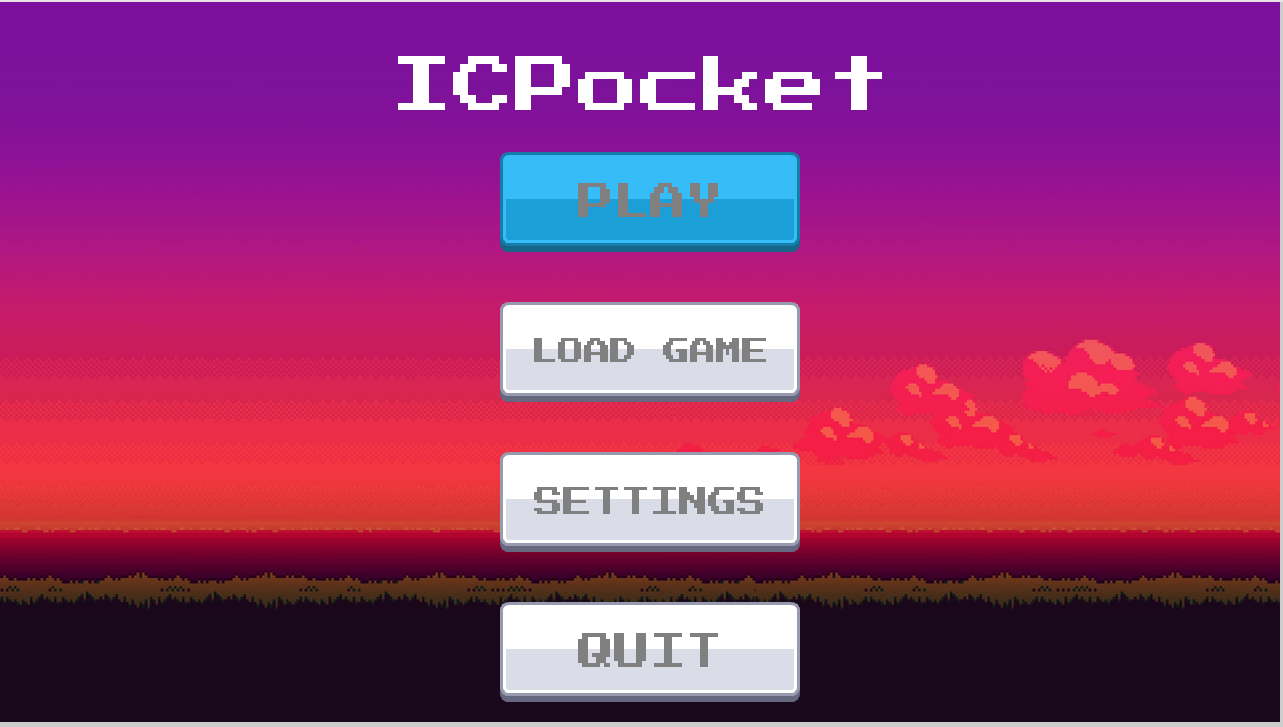
\includegraphics[width=\textwidth]{menuicmonp.png}
            \caption{Menu principal du jeu ICPocket}
            \label{fig:menuicmonp}
        \end{minipage}
        \hfill
        \begin{minipage}[t]{0.48\textwidth}
            \centering
            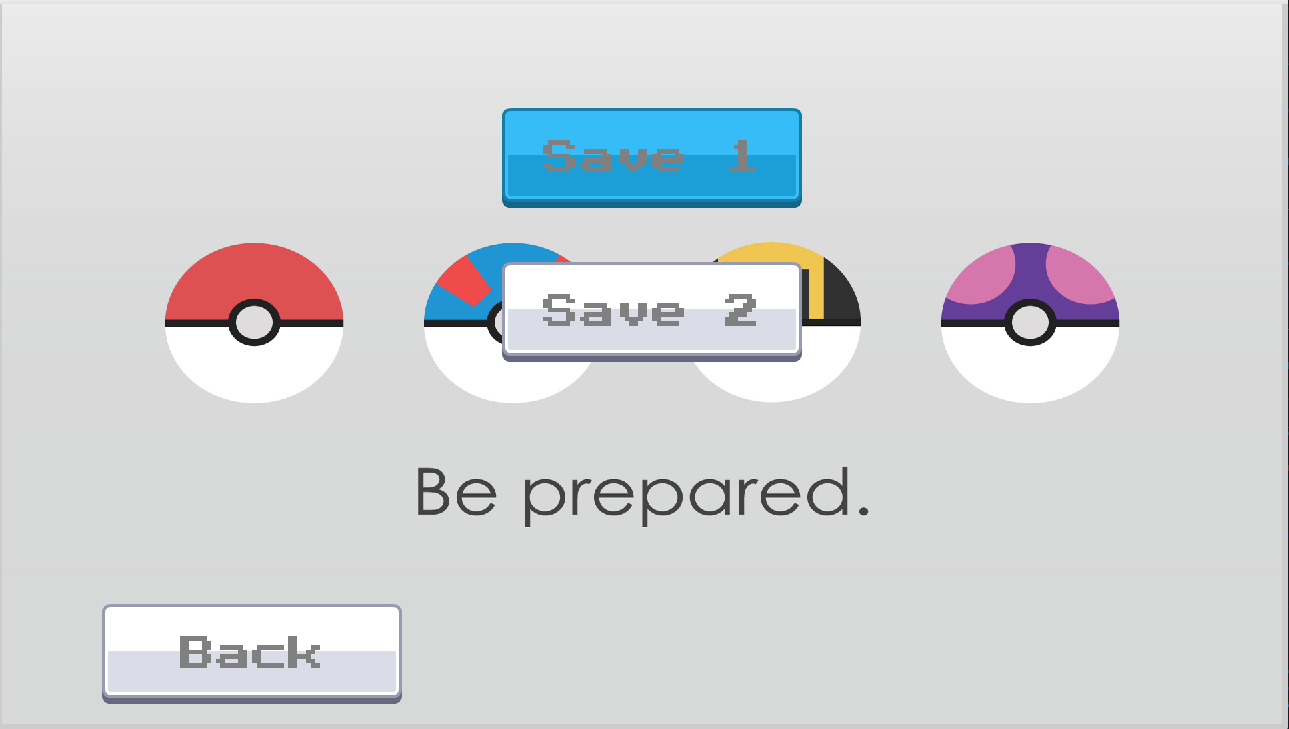
\includegraphics[width=\textwidth]{menuload.png}
            \caption{Menu de chargement du jeu ICPocket}
            \label{fig:menuload}
        \end{minipage}
    \end{figure}
    \paragraph{} \emph{Dans le code, les fonctions de sauvegarde et de chargement se situent dans le fichier \texttt{save.c}.}
    \paragraph{} \textbf{sauvegarder} prend comme paramètres des structures d'équipes , respectivement celui du joueur et celui de l'adversaire,
    et cherche le fichier correspondant au numéro du bouton de sauvegarde appuyé. Ensuite , enregistre seulement les numéros d'identification des ICMons et leurs caractéristiques générés aléatoirement ou choisis par le joueur, telles que les IVs,niveaux de ICmon , le nombre et type d'attaque. Enfin,elle sauvegarde les données liées a la progression
    comme le nombre de joueurs battus et leurs pseudo.
    \paragraph{} \textbf{charger} prend comme paramètres le numéro de sauvegarde et la structure d'équipe du joueur. Elle ouvre le fichier CSV
    correspondant et lit les données ligne par ligne en suivant le format défini par la fonction précédente. si 

    \subsubsection{base de données des icmons}
    Toutes la gestion de base de données ont été fais dans des fichiers CSV situés dans le dossier \texttt{data/}
    Les ICMons sont générés grâce a leurs ID leurs numéro d'identification, avec la fonction \texttt{generate\_poke} et \texttt{generate\_poke\_ennemie} qui prennent donc en paramètres les ID.

      
\newpage
\subsection{Gestion de la map}

    \subsubsection{Chargement de la map}
    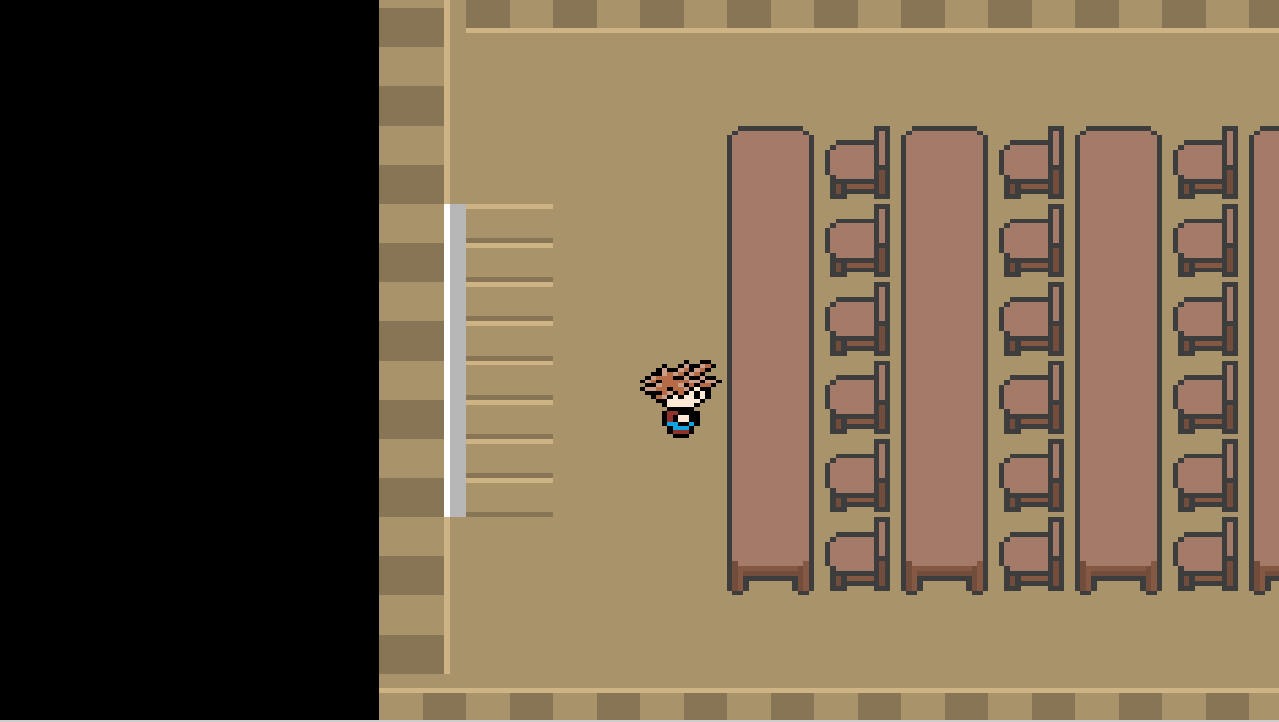
\includegraphics[width=0.8\textwidth]{../docs/img/screenshots/screen2.png}
    \newline
    \paragraph{Analyse : }
   
    Pour améliorer la qualité de notre gameplay et la qualité visuelle de notre jeu, nous avons décidé de créer une carte en 2D qui reconstitue le rez-de-chaussée de l'IC2, où nous pouvons retrouver des
    zones existantes du bâtiment telles que l'amphithéâtre, comme l'image ci-dessus. L'utilisation de fichiers CSV a permis de gérer les collisions. Dans les fichiers, les numéros 1 correspondent 
    aux collisions, les 0 aux zones libres où le personnage peut marcher, et d'autres numéros servent à passer d'une carte à l'autre, comme du hall à l'amphithéâtre, grâce à une lecture de fichier qui permet
    de reconnaître l'endroit où l'on va. La carte apporte une plus grande liberté dans le jeu puisqu'il y a la possibilité de se déplacer partout dans le bâtiment. Il y a également l'ajout d'un PNJ
    (personnage non joueur) qui permet à l'utilisateur de lancer les combats dans l'ordre donné. 
    \newline
    \paragraph{Réalisation : }
    Pour finir sur le chargement de la carte, il y a eu la création de points de spawn qui sont accordés au chiffre -1, les collisions aux chiffres 1 et les zones libres aux 0 dans nos fichiers CSV. 
    Voici un exemple de CSV correspondant à l'amphithéâtre :
    \begin{center}
    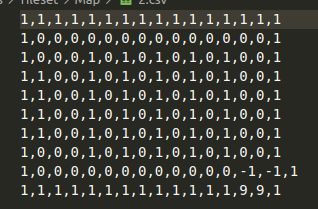
\includegraphics[width=0.5\textwidth]{hall.png}
    \end{center}
    \begin{center}
        \small{-1=spawn 0=Air 1=collision 9=retour dans le hall.}
    \end{center}
    
    Les fonctions implémentées afin de rendre le rendu de la carte possible sont `initMap`, qui permet d'initialiser la carte en utilisant les autres fonctions du fichier `Map.c`, telles que `initCollisionFromCSV`,
    qui permet de gérer les collisions grâce aux CSV. Nous avons créé la fonction `checkAndLoadNewMap`, qui permet de vérifier si, dans un fichier CSV, le personnage se situe sur une case qui correspond au chargement d'une nouvelle zone. Dans ce cas, 
    la fonction 'loadNewMap' est appelée pour mettre à jour le point d'apparition du joueur par rapport à la nouvelle carte et lorsque le joueur revient sur la carte précédente, il est renvoyé à l'endroit où il était avant de changer de zone.
    Pour ce faire, le programme regarde dans ses plus proches voisins s'il y a une case 0, si oui le joueur est directement placé à cet endroit.

    Pour rendre cela possible, nous avons utilisé le logiciel de création de carte Tiled, puis Aseprite pour rendre la carte plus jolie en retirant les impuretés, afin de gérer tout cela avec des fichiers CSV.
    Tiled permet de créer des cartes facilement et de les exporter au format CSV, ce qui simplifie leur intégration dans le jeu.
    \subsubsection{Caméra}
    La gestion de la caméra est un élément essentiel pour offrir une expérience utilisateur fluide et immersive dans notre jeu. La caméra permet de suivre les déplacements du joueur tout en affichant une partie de la map grâce au zoom, ce qui est particulièrement utile pour les grandes cartes en 2D. Cela évite d'afficher l'intégralité de la map à l'écran, ce qui pourrait surcharger visuellement le joueur et réduire les performances.
    \paragraph{Utilité de la caméra :} La caméra a été implémentée pour plusieurs raisons :
    Suivi du joueur : La caméra suit dynamiquement la position du joueur, garantissant que ce dernier reste toujours visible à l'écran.
    La map est rendue en entier puis fait un zoom sur le joueur afin de le suivre uniquement et cacher l'affichage des endroits inutiles.

    Immersion : En limitant la vue du joueur à une zone spécifique, la caméra renforce l'immersion en simulant une perspective réaliste.

    \paragraph{Pourquoi l'avoir implémentée ?}

    L'implémentation de la caméra était nécessaire pour gérer efficacement les grandes maps et offrir une meilleure expérience utilisateur. Sans caméra, il aurait été impossible de naviguer correctement sur des cartes de grande taille, car tout serait affiché en même temps, rendant le jeu confus et peu ergonomique. De plus, la caméra permet de centrer l'attention du joueur sur son personnage et les zones importantes, tout en masquant les parties inutiles de la map.
    Nous avons donc utilisé le système d'interpolation linéaire pour avoir un rendu pixel par pixel.
    La caméra a été conçue pour être flexible et s'adapter à différentes tailles de fenêtres.

    En résumé, la caméra joue un rôle crucial dans la navigation et le rendu du jeu, en améliorant à la fois les performances et l'expérience utilisateur.
    Tout cela a été possible grâce aux différents outils utilisés tels que Stack Overflow, Developpez.net, Wikipedia afin d'utiliser l'interpolation linéaire.
    \paragraph{Réalisation : }
    L'utilisation de fonctions était obligatoire pour bien gérer la caméra. Pour cela, la fonction `getWorldToScreenRect` permet de convertir les coordonnées du monde en coordonnées écran.
    `updateCameraViewport` permet de mettre à jour la taille visible de la carte par rapport à la caméra et `updateCamera` fait en sorte d'actualiser la position de la caméra grâce à l'utilisation de l'interpolation linéaire,
    ce qui permet un rendu plus fluide des déplacements du joueur.

    \newpage
    \subsubsection{Déplacement}

    Dans un jeu, les déplacements sont les choses les plus importantes puisque sans ça, on ne peut rien faire sur une carte.

    \paragraph{Implémentation des fonctions : }

    Pour gérer les déplacements du joueur, nous utilisons la fonction `createPlayer`, qui a pour but de créer le joueur et son sprite (image) ainsi que de définir comment il va se déplacer. Dans cette fonction, les déplacements se font par des calculs de coordonnées afin de déplacer le joueur du point de spawn jusqu'à la prochaine case, que ce soit en haut, en bas, à gauche ou à droite, à condition de ne pas rencontrer de collision.
    \newline

    Pour déplacer le joueur ainsi que gérer les animations du sprite, il faut utiliser les fonctions `updatePlayerPosition` et `updatePlayerAnimation`. La fonction `updatePlayerPosition` met à jour la position du joueur sur la carte en utilisant un système d'interpolation linéaire pour rendre les déplacements fluides. Elle calcule la position intermédiaire entre la position actuelle et la position cible en fonction du temps écoulé (`deltaTime`).
    \newline

    La fonction `updatePlayerAnimation` permet de changer le sprite du joueur en fonction de son état (marche vers le haut, le bas, la gauche ou la droite). Elle utilise un système de frames pour donner un style d'animation réaliste, en alternant entre différentes images de la spritesheet.
    \newline

    L'ajout des déplacements donne une sorte de liberté au jeu, où le personnage peut se déplacer où il veut sur la carte. Grâce aux animations du personnage, cela rend les déplacements encore plus immersifs et réalistes.
    \newline

    De plus, la fonction `renderPlayerWithCamera` est utilisée pour afficher le joueur à l'écran en tenant compte de la position de la caméra. Cela permet de s'assurer que le joueur reste visible même lorsque la carte est plus grande que la fenêtre d'affichage.
    \newline

    Enfin, les déplacements sont également liés à la gestion des collisions. Le joueur ne peut se déplacer que sur des cases libres (valeurs spécifiques dans la matrice de la carte). Cela est vérifié dans les fonctions de gestion des événements, comme `handlePlayerEvent`, qui détecte les entrées clavier et met à jour l'état du joueur en conséquence.

\newpage
\subsection{rendu du jeu}
Le système de rendu graphique constitue l'un des piliers fondamentaux de notre jeu, devant concilier performances optimales et cohérence visuelle.

\paragraph{Architecture de base} Notre implémentation repose sur la bibliothèque SDL (Simple DirectMedia Layer) qui offre une couche d'abstraction multiplateforme pour l'accès au matériel graphique. Pour garantir une expérience fluide malgré la richesse visuelle du jeu, nous avons développé une architecture de rendu multi-niveaux qui sépare les différentes composantes graphiques.

\paragraph{Gestion des threads} Une caractéristique notable de notre moteur de rendu est son intégration avec un système multi-thread. Notre gestionnaire de threads initialise plusieurs verrous mutex dédiés aux ressources partagées : l'audioMutex pour les opérations sonores, le physicsMutex pour les calculs de déplacement et collisions, et initialement un renderMutex pour les opérations graphiques (désactivé dans la version finale pour des raisons d'optimisation).

Cette approche multi-thread permet d'exécuter simultanément la logique du jeu et le rendu graphique, optimisant ainsi l'utilisation des ressources système. Le rendu spécifique de la carte du monde est effectué dans une fonction dédiée (renderMap) qui synchronise l'accès aux données partagées à l'aide de mutex. Cette fonction verrouille d'abord le mutex physique, effectue les opérations de rendu de la carte et du joueur avec la caméra, puis déverrouille le mutex avant de présenter le résultat à l'écran.

La gestion des images par seconde (FPS) est assurée par un mécanisme sophistiqué (manageFrameRate) qui ajuste dynamiquement le timing du rendu pour maintenir une cadence constante. Notre système vise un objectif de 60 FPS en calculant le temps écoulé depuis le début de la frame et en introduisant un délai approprié si nécessaire. Ce mécanisme garantit une expérience fluide tout en calculant précisément le deltaTime, une variable critique pour la synchronisation des animations et des mouvements indépendamment de la puissance de calcul disponible.

\subsubsection{gestion de l'interface}
\paragraph{Système d'états} Notre interface utilisateur est gérée par un système d'états (définis dans l'énumération AppState) qui détermine quels éléments doivent être affichés à chaque instant. La fonction render orchestre l'affichage des différents composants en fonction de l'état actuel du jeu. Cette fonction conditionne le rendu selon des valeurs telles que MENU, NEWGAME, SWAP, LEARNMOVE ou STARTERS, appelant les fonctions de rendu appropriées pour chaque situation.

\paragraph{Transitions et mises à jour} Les transitions entre ces différents états sont gérées par une fonction changeState qui assure la cohérence des données et prépare les ressources nécessaires au nouvel état. Cette fonction prend en compte à la fois l'état actuel et l'état cible pour effectuer les actions de transition appropriées, comme l'initialisation d'un combat lorsque l'on passe de l'exploration à un affrontement.

\paragraph{Mise à jour des textes des boutons} La fonction updateICMonsButtonText parcourt l'équipe spécifiée et met à jour les textes des boutons correspondants dans l'interface utilisateur. Si un emplacement est vide, le bouton affiche un espace, sinon il affiche le nom de l'ICMon. Ce système permet de maintenir une cohérence visuelle même lorsque les données sous-jacentes changent, comme lors d'un échange d'ICMons ou de l'apprentissage de nouvelles capacités.

\paragraph{Gestion des événements} La gestion des événements utilisateur est assurée par un ensemble de fonctions spécialisées pour chaque état du jeu, comme handleLoadGameEvent ou handlePauseEvent, qui interprètent les interactions et déclenchent les actions appropriées. Par exemple, la fonction de gestion des pauses vérifie si la touche Échap a été pressée et change l'état du jeu en conséquence.

\subsubsection{gestion des combats avec SDL}
\paragraph{Machine à états} Le système de combat repose sur une machine à états finie représentée par l'énumération BattleTurnState, qui définit les différentes phases d'un tour : initialisation (TURN\_INIT), attente des instructions du joueur (TURN\_WAIT\_TEXT), exécution des actions (TURN\_ACTION1 et TURN\_ACTION2), et finalisation (TURN\_FINISHED).

\paragraph{Rendu des sprites} Le rendu des sprites des ICMons est géré par des fonctions spécialisées comme renderICMonsSprite, qui s'occupe de positionner et d'animer correctement les créatures à l'écran. L'initialisation des sprites est effectuée lors du chargement d'une partie par la fonction initTeamSprites, qui prend en compte le positionnement relatif des sprites sur l'écran, avec des ratios différents selon qu'il s'agit de l'équipe du joueur (BLUE SPRITE X RATIO, BLUE SPRITE Y RATIO) ou de l'adversaire (RED SPRITE X RATIO, RED SPRITE Y RATIO).

\subsubsection{Optimisation des performances}
\paragraph{Gestion des ressources} Notre moteur de rendu inclut plusieurs mécanismes d'optimisation pour garantir des performances fluides. L'un des plus importants est la gestion des ressources lors des transitions entre états. Lorsqu'un joueur passe de l'exploration à un combat, ou lors d'un changement de map, nous devons libérer certaines ressources et en charger d'autres. Cette gestion est centralisée dans la fonction cleanupResources qui libère méthodiquement les textures, les textes, les contrôleurs et les structures de données comme la carte, le joueur et la caméra.

\paragraph{Orchestration des threads} Un autre aspect critique de l'optimisation est l'orchestration des threads. En séparant la logique audio, la physique et le rendu dans des threads distincts, nous exploitons efficacement les architectures multi-cœurs modernes.

La fonction principale du jeu (mainLoop) coordonne l'ensemble du processus de rendu en gérant les événements, en appelant les fonctions de rendu appropriées selon l'état du jeu, et en maintenant une cadence constante grâce à manageFrameRate. Cette boucle distingue le cas spécial de l'état MAP, où elle utilise renderMap, des autres états où elle effectue un rendu standard avec gestion des boutons et mise à jour du tour de combat si nécessaire.

En conclusion, notre système de rendu combine une architecture multi-thread sophistiquée, une gestion d'états flexible et des mécanismes d'optimisation ciblés pour offrir une expérience visuelle riche tout en maintenant des performances fluides sur une variété de configurations matérielles. Ce système démontre l'efficacité de notre approche modulaire et la pertinence de nos choix techniques, notamment l'utilisation de SDL et la parallélisation des traitements.

\subsubsection{Technologies graphiques et défis techniques}
\paragraph{Synchronisation} L'implémentation de notre système de rendu a nécessité de relever plusieurs défis techniques spécifiques. L'un des plus complexes concernait la synchronisation entre le système de rendu et le système de physique, particulièrement critique lors des transitions entre maps. Nous avons conçu un mécanisme de verrouillage sélectif qui permet au thread physique de continuer à calculer les collisions et les déplacements pendant que le thread principal s'occupe du rendu, tout en évitant les problèmes de concurrence.

\paragraph{Effets visuels} Le rendu des effets visuels dynamiques, comme les animations d'attaque ou les transitions entre états du jeu, a également posé des défis techniques significatifs. Nous avons implémenté un système de timers et de séquences qui permet de coordonner précisément les animations avec la logique du jeu. Ce système utilise le deltaTime calculé par notre gestionnaire de fréquence d'images pour garantir une vitesse d'animation cohérente quelle que soit la puissance de calcul disponible.

\paragraph{Adaptabilité} Un autre aspect innovant de notre système graphique est la gestion adaptative de la qualité visuelle. Sur les configurations matérielles moins puissantes, notre moteur peut automatiquement réduire certains effets visuels pour maintenir une fréquence d'images acceptable. Cette adaptation dynamique est particulièrement importante pour notre jeu qui vise une large compatibilité matérielle.

Le rendu des textes a également bénéficié d'une attention particulière, avec un système de mise en cache des textures de texte pour éviter de régénérer constamment les mêmes chaînes de caractères. Cette optimisation s'est révélée particulièrement efficace dans les écrans de combat où les mêmes messages peuvent apparaître à plusieurs reprises.

Notre approche du rendu multi-couches, particulièrement visible dans les écrans de combat, permet de composer des scènes visuellement riches en combinant différents éléments (arrière-plans, sprites des créatures, interface utilisateur) avec un contrôle précis sur l'ordre de dessin. Cette technique garantit que les éléments sont toujours affichés dans le bon ordre, évitant les problèmes de superposition incorrecte.

Pour conclure, l'architecture de notre système de rendu, bien que développée avec des technologies relativement simples comme SDL, démontre qu'une conception réfléchie et une implémentation soignée peuvent conduire à des résultats visuellement impressionnants et techniquement efficaces. Notre approche modulaire facilite également l'extension future du moteur avec de nouvelles fonctionnalités visuelles sans nécessiter de refonte majeure du système existant.
\newpage
\section{Bilan et résultats}

\subsection{Bilan}
Le projet a été un succès, tant sur le plan technique que sur le plan de l'expérience utilisateur. Nous avons réussi à créer un jeu 2D fonctionnel et agréable à jouer, avec une interface intuitive et des mécaniques de jeu inspirées de l'univers Pokémon. La gestion des ICMons, des combats et des déplacements a été bien intégrée, offrant une expérience fluide et immersive.
La répartition des tâches a été efficace, chaque membre de l'équipe ayant pu contribuer selon ses compétences et ses intérêts. La communication constante entre les membres a permis d'identifier rapidement les problèmes et de trouver des solutions adaptées.
Nous avons également appris à travailler avec des outils de développement modernes, tels que GitHub pour la gestion de version, et à utiliser des ressources en ligne pour résoudre des problèmes techniques. L'utilisation de GitHub Copilot a été un atout précieux pour accélérer le développement et améliorer la qualité du code.

\subsection{Résultats}
Les résultats obtenus sont plus que satisfaisants grâce aux différents ajouts et améliorations apportés au projet. Nous avons ajouté de la liberté grâce à la carte et aux PNJ. Toutes les modifications apportées et l'avancement plus rapide du projet ont donc modifié notre Gantt prévisionnel pour en arriver au Gantt final ci-dessous.
\begin{figure}[h]
    \centering
    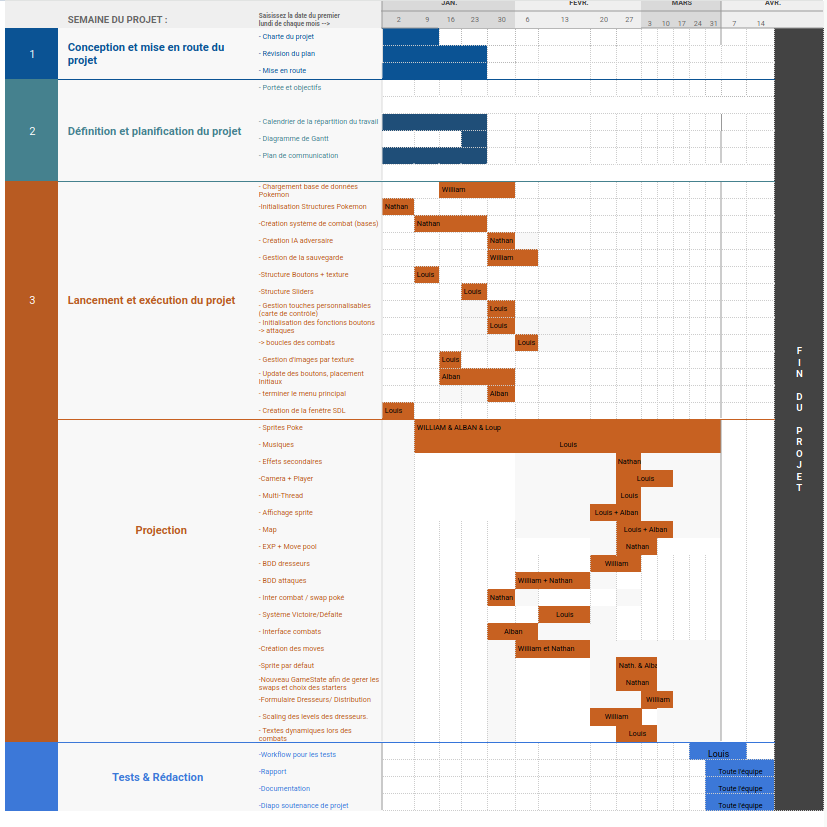
\includegraphics[width=0.75\textwidth]{gantt finale.png}
    \label{fig:GANTT}
    \caption{Diagramme de Gantt}
\end{figure}
\subsection{Avis des membres de l'équipe sur le projet}
Avis des membres de l'équipe :
\begin{itemize}
    \item \textbf{Alban :} « J'ai énormément apprécié réaliser ce projet avec mon groupe car nous avons eu une très bonne entente directement, que ce soit la répartition des tâches ou la communication entre nous. Nous avons tous su nous entraider et nous conseiller sur les différentes parties du projet. De plus, j'ai beaucoup appris sur le développement de jeux vidéo, notamment sur le fait d'approfondir mes capacités en C et de découvrir la bibliothèque SDL. J'ai également appris à utiliser GitHub. Je suis très satisfait du résultat final et j'espère que nous pourrons continuer à développer d'autres projets ensemble ».
    \newline
    \item \textbf{Louis :} J'ai beaucoup aimé réaliser ce projet de fin d'année avec mon groupe. Nous qui étions déjà très proches, avons pu nous mettre d'accord sur les différentes parties du projet et nous avons pu nous entraider. J'ai également appris beaucoup de choses sur le développement de jeux vidéo, notamment sur le fait d'approfondir mes capacités en C et de découvrir la bibliothèque SDL. Si je devais recommencer ce projet, je changerais certaines choses, comme la gestion des threads et des ressources, afin de rendre le jeu encore plus fluide et performant, j'ai aussi appris à structurer correctement un projet petit à petit donc ce serait aussi une bonne chose à améliorer.
    \newline
    \item \textbf{Nathan :} En tant que fan absolu de \emph{Pokémon}, j'ai personnellement adoré réaliser ce projet. La cohésion dans le groupe ne pouvait être meilleure, et par conséquent le résultat est parfaitement à la hauteur de mes attentes. De plus, ceci fût ma première expérience de réalisation de projet de grande envergure mais également de réalisation de jeux vidéos et de travail en équipe, ce qui m'a permis d'enrichir mes connaissances en vue de mon parcours professionnels à venir.
    \newline
    \item \textbf{William :} Réaliser ce projet a été une expérience enrichissante, tant sur le plan technique que sur la gestion de l'organisation. La communication et la répartition des taches ont été facilitées car nous sommes tous au courant des compétences et limites de chacuns, puisque que nous nous entendions très bien en dehors des cours. Sur le plan personnel j'ai appris a utilisé github qui est un élément essentiel pour un développeur voulant travailler en équipe, j'ai aussi expérimenté les difficultés et les opportunités rencontrées lorsqu'une équipe créer un projet de cet envergure. Mes compétences en C ont été mises à l'épreuve pour une derniere fois avant la fin d'année, ce qui m'a permis de les améliorer considérablement.
    
\end{itemize}
\section{Références}
\subsection{Outils de développement}
\label{annexe:github}
\textbf{GitHub :} \href{https://github.com/Lounol72/ICPocket}{github.com}

\label{annexe:stackoverflow}
\textbf{Stack Overflow :} \href{https://stackoverflow.com/questions/tagged/sdl}{stackoverflow.com}

\label{annexe:bulbapedia}
\textbf{Bulbapedia :} \href{https://bulbapedia.bulbagarden.net/wiki}{bulbapedia.bulbagarden.net}

\label{annexe:showdown}
\textbf{PokemonShowdown Calc :} \href{https://calc.pokemonshowdown.com}{calc.pokemonshowdown.com}

\label{annexe:developpez}
\textbf{Developpez.net :} \href{https://forum.developpez.com}{forum.developpez.com}

\label{annexe:copilot}
\textbf{GitHub Copilot :} \href{https://copilot.github.com/}{copilot.github.com}

\label{annexe:aseprite}
\textbf{Aseprite :} \href{https://www.aseprite.org/}{aseprite.org}

\label{annexe:tiled}
\textbf{Tiled :} \href{https://www.mapeditor.org/}{mapeditor.org}

\label{annexe:pokepedia}
\textbf{Poképédia :} \href{https://www.pokepedia.fr/}{pokepedia.fr}

\section{Annexes}



\end{document}